% A LaTeX template for EXECUTIVE SUMMARY of the MSc Thesis submissions to
% Politecnico di Milano (PoliMi) - School of Industrial and Information Engineering
%
% P. F. Antonietti, S. Bonetti, A. Gruttadauria, G. Mescolini, A. Zingaro
% e-mail: template-tesi-ingind@polimi.it
%
% Last Revision: October 2021
%
% Copyright 2021 Politecnico di Milano, Italy. Inc. All rights reserved.

\documentclass[11pt,a4paper]{article}

%------------------------------------------------------------------------------
%	REQUIRED PACKAGES AND  CONFIGURATIONS
%------------------------------------------------------------------------------
% PACKAGES FOR TITLES
\usepackage{titlesec}
\usepackage{color}
% PACKAGES FOR LANGUAGE AND FONT
\usepackage[utf8]{inputenc}
\usepackage[english]{babel}
\usepackage[T1]{fontenc} % Font encoding
\usepackage{lmodern} % Latin Modern font
% PACKAGES FOR IMAGES
\usepackage{graphicx}
\graphicspath{{Images/}} % Path for images' folder
\usepackage{eso-pic} % For the background picture on the title page
\usepackage{subfig} % Numbered and caption subfigures using \subfloat
\usepackage{caption} % Coloured captions
%\usepackage{subcaption}
\usepackage{transparent}


% STANDARD MATH PACKAGES
\usepackage{amsmath}
\usepackage{amsthm}
\usepackage{bm}
\usepackage[overload]{empheq}  % For braced-style systems of equations

% PACKAGES FOR TABLES
\usepackage{tabularx}
\usepackage{longtable} % tables that can span several pages
\usepackage{colortbl}

% PACKAGES FOR ALGORITHMS (PSEUDO-CODE)
\usepackage{algorithm}
\usepackage{algpseudocode}
% PACKAGES FOR REFERENCES & BIBLIOGRAPHY
\usepackage[maxbibnames=99]{biblatex}
\addbibresource{mimesis.bib}
\usepackage[colorlinks=true,linkcolor=black,anchorcolor=black,citecolor=black,filecolor=black,menucolor=black,runcolor=black,urlcolor=black]{hyperref} % Adds clickable links at references
\usepackage{cleveref}
%\usepackage[square, numbers, sort&compress]{natbib} % Square brackets, citing references with numbers, citations sorted by appearance in the text and compressed
\usepackage{bookmark} % Add this package to fix the reported errors
% \bibliographystyle{plain} % You may use a different style adapted to your field
% \bibliographystyle{plain} % You may use a different style adapted to your field

% PACKAGES FOR THE APPENDIX

\usepackage{appendix}

% PACKAGES FOR ITEMIZE & ENUMERATES
\usepackage{enumitem}

% OTHER PACKAGES
\usepackage{amsthm,thmtools,xcolor} % Coloured "Theorem"
\usepackage{comment} % Comment part of code
\usepackage{fancyhdr} % Fancy headers and footers
\usepackage{lipsum} % Insert dummy text
\usepackage{tcolorbox} % Create coloured boxes (e.g. the one for the key-words)
\usepackage{stfloats} % Correct position of the tables
\usepackage{multirow}
\usepackage{multicol}






%-------------------------------------------------------------------------
%	NEW COMMANDS DEFINED
%-------------------------------------------------------------------------
% EXAMPLES OF NEW COMMANDS -> here you see how to define new commands
\newcommand{\bea}{\begin{eqnarray}} % Shortcut for equation arrays
\newcommand{\eea}{\end{eqnarray}}
\newcommand{\e}[1]{\times 10^{#1}}  % Powers of 10 notation
\newcommand{\mathbbm}[1]{\text{\usefont{U}{bbm}{m}{n}#1}} % From mathbbm.sty
\newcommand{\pdev}[2]{\frac{\partial#1}{\partial#2}}
% NB: you can also override some existing commands with the keyword \renewcommand

%----------------------------------------------------------------------------
%	ADD YOUR PACKAGES (be careful of package interaction)
%----------------------------------------------------------------------------
\usepackage{amsfonts} 
\usepackage[font=footnotesize,labelfont=bf]{caption}
\usepackage{placeins} % in your preamble


%----------------------------------------------------------------------------
%	ADD YOUR DEFINITIONS AND COMMANDS (be careful of existing commands)
%----------------------------------------------------------------------------
\usepackage{import}
\usepackage{xifthen}
\usepackage{pdfpages}
\usepackage{transparent}
\usepackage{wrapfig}
\usepackage{dsfont}
\usepackage{shadethm}
\usepackage{tikz}
\usetikzlibrary{positioning}

\def\layersep{2.5cm}

\parindent=0pt

\newcommand{\incfig}[1]{%
    \def\svgwidth{\columnwidth}
    \import{./Images/}{#1.pdf_tex}
}
\newcommand*{\oldepsilon}{\epsilon}
\renewcommand*{\epsilon}{\varepsilon}
\newcommand*{\oldphi}{\phi}
\renewcommand*{\phi}{\varphi}
\DeclareMathOperator*{\esssup}{ess\,sup}
\DeclareMathOperator*{\argmax}{arg\,max}
\DeclareMathOperator*{\argmin}{arg\,min}

\numberwithin{equation}{section}
%----------------------------------------------------------------------------
%	CONFIGURATION OF THEOREM ENVIRONMENTS


% \newtheoremstyle{break}
%     {\partopsep}{\topsep}%  
%     {\normalfont}{}
%     {\bfseries}{}%
%     {\newline}{}%
% \theoremstyle{break}
% \newtheorem{theorem}{Theorem}[section]
% \newtheorem{corollary}{Corollary}[section]
% \newtheorem{proposition}{Proposition}[section]
% \newtheorem{remark}{Remark}[section]
% \newtheorem{lemma}{Lemma}[section]
% \newtheorem{notation}{Notation}[section]
% \newtheorem{definition}{Definition}[section]

% \newtheorem{definition}{Definition}[section]

% \newtheorem*{remark}{Remark}

% \newtheorem{lemma}{Lemma}[section]
% %----------------------------------------------------------------------------

% Do not change Configuration_files/config.tex file unless you really know what you are doing.
% This file ends the configuration procedures (e.g. customizing commands, definition of new commands)
% Set the geometric layout of the document
\usepackage{geometry}
\geometry{
  top=3cm,
  left = 2.0cm,
  right = 2.0cm,
  bottom=2cm,
  headheight= 2cm,
  headsep= 0cm,
}
\raggedbottom

% Create color bluePoli (-> manuale grafica coordinata:  https://www.polimi.it/fileadmin/user_upload/il_Politecnico/grafica-coordinata/2015_05_11_46xy_manuale_grafica_coordinata.pdf)
\definecolor{bluePoli}{cmyk}{0.4,0.1,0,0.4}

% Custom theorem environments
\declaretheoremstyle[
  shaded={rulecolor=bluePoli!20, rulewidth=1pt, bgcolor=bluePoli!5},
  headfont=\color{bluePoli}\normalfont\bfseries,
  bodyfont=\color{black}\normalfont,
]{colored}

\captionsetup[figure]{labelfont={color=bluePoli}} % Set colour of the captions
\captionsetup[table]{labelfont={color=bluePoli}} % Set colour of the captions
\captionsetup[algorithm]{labelfont={color=bluePoli}} % Set colour of the captions

\theoremstyle{colored}
\newtheorem{theorem}{Theorem}[section]
\newtheorem{proposition}{Proposition}[section]
\newtheorem{definition}{Definition}[section]
\newtheorem*{remark}{Remark}
\newtheorem{lemma}{Lemma}[section]

% Enhances the features of the standard "table" and "tabular" environments.
\newcommand\T{\rule{0pt}{2.6ex}}
\newcommand\B{\rule[-1.2ex]{0pt}{0pt}}

% Algorithm description
\newcounter{algsubstate}
\renewcommand{\thealgsubstate}{\alph{algsubstate}}
\newenvironment{algsubstates}{
    \setcounter{algsubstate}{0}%
    \renewcommand{\STATE}{%
    \stepcounter{algsubstate}%
    \Statex {\small\thealgsubstate:}\space}
    }{}

% Custom theorem environment
\newcolumntype{L}[1]{>{\raggedright\let\newline\\\arraybackslash\hspace{0pt}}m{#1}}
\newcolumntype{C}[1]{>{\centering\let\newline\\\arraybackslash\hspace{0pt}}m{#1}}
\newcolumntype{R}[1]{>{\raggedleft\let\newline\\\arraybackslash\hspace{0pt}}m{#1}}

% Custom itemize environment
\setlist[itemize,1]{label=$\bullet$}
\setlist[itemize,2]{label=$\circ$}
\setlist[itemize,3]{label=$-$}
\setlist{nosep}

% Set separation of columns
\setlength{\columnsep}{30pt}

% Create command for background pic
\newcommand\BackgroundPic{% Adding background picture
	\put(230,358){
		\parbox[b][\paperheight]{\paperwidth}{%
			\vfill
			\centering
			\transparent{0.2}
			
\includegraphics[width=0.8\paperwidth]{raggiera_polimi.eps}%
			\vfill
}}}

% Set indentation
%\setlength\parindent{0pt}

% Custom title commands
\titleformat{\section}
{\color{bluePoli}\normalfont\Large\bfseries}
{\color{bluePoli}\thesection.}{1em}{}
\titlespacing*{\section}
{0pt}{2ex}{1ex}

\titleformat{\subsection}
{\color{bluePoli}\normalfont\large\bfseries}
{\color{bluePoli}\thesubsection.}{1em}{}
\titlespacing*{\subsection}
{0pt}{2ex}{1ex}

\titleformat{\subsubsection}
{\color{bluePoli}\normalfont\normalsize\bfseries}
{\color{bluePoli}\thesubsubsection.}{1em}{}
\titlespacing*{\subsubsection}
{0pt}{2ex}{1ex}

% Custom headers and footers
\pagestyle{fancy}
\fancyhf{}

\fancyfoot{}
\fancyfoot[C]{\thepage} % page
\renewcommand{\headrulewidth}{0mm} % headrule width
\renewcommand{\footrulewidth}{0mm} % footrule width

\makeatletter
\patchcmd{\headrule}{\hrule}{\color{black}\hrule}{}{} % headrule
\patchcmd{\footrule}{\hrule}{\color{black}\hrule}{}{} % footrule
\makeatother

% -> Create the header
\chead[C]{
\centering
\begin{tcolorbox}[arc=0pt, boxrule=0pt, colback=bluePoli!60, width=\textwidth, colupper=white]
    
\includegraphics[width=0.2\textwidth]{mimesis.png}
\end{tcolorbox}
}


% Insert here the info that will be displayed into your Title page
% -> title of your work
\renewcommand{\title}{\noindent A Modified Neural Modes Approach for Soft Tissue Simulation}


% -> author name and surname
\renewcommand{\author}{Andrea Bonifacio}
% -> student ID
\newcommand{\ID}{217658} % insert your student ID here
% -> MSc course
\newcommand\norm[1]{\lVert#1\rVert}
\newcommand{\course}{Mathematical Engineering - Ingegneria Matematica}
% -> advisor name and surname
\newcommand{\advisor}{Prof. Stefano Pagani}
% IF AND ONLY IF you need to modify the co-supervisors you also have to modify the file Configuration_files/title_page.tex (ONLY where it is marked)
\newcommand{\firstcoadvisor}{Dr. Stéphane Cotin} % insert if any otherwise comment
%\newcommand{\secondcoadvisor}{Name Surname} % insert if any otherwise comment
% -> academic year
\newcommand{\YEAR}{2024-2025}

\renewcommand{\abstract}{This thesis investigate a model order reduction approach to address the computational challenges of simulating the dynamic, nonlinear deformation of soft tissues, particularly when using traditional Finite Element Methods (FEM). We first investigate the efficiency and accuracy of the Neural Modes method, developed by Wang et al. \cite{Wang_Du_Coros_Thomaszewski_2024}. The core of the method trains a deep neural network to learn nonlinear corrections to a reduced-order linear modal basis. This approach not only accelerates simulations by operating in a reduced-dimensional space but also enhances the interpretability of the learned model, as the corrections are applied to linear modes. Building upon their ideas, we develop a simulation framework that combines the computation of the energy during the training of the network, keeping the physics-informed loss function, with a supervised learning strategy that allows the network to learn nonlinear corrections for large deformations. 
The efficacy of the Neural Modes framework is demonstrated through numerical experiments on some 3D benchmark problems, showcasing its potential for applications in biomechanics and surgical simulation where both speed and accuracy are fundamental.
}

\newcommand{\abstractita}{Questa tesi studia un approccio tramite modelli a ordine ridotto per affrontare le sfide computazionali della simulazione della deformazione dinamica e non lineare dei tessuti molli, in particolare quando si utilizzano i tradizionali metodi agli elementi finiti (FEM). In primo luogo, esaminiamo l'efficienza e l'accuratezza del metodo Neural Modes, sviluppato da Wang et al. \cite{Wang_Du_Coros_Thomaszewski_2024}. Alla base del metodo vi è l'addestramento di una rete neurale per apprendere correzioni non lineari rispetto a una base modale lineare di ordine ridotto. Questo approccio non solo accelera le simulazioni operando in uno spazio di dimensioni ridotte, ma migliora anche l'interpretabilità del modello, poiché le correzioni sono applicate a modalità lineari. Sulla base delle loro idee, sviluppiamo un framework di simulazione che combina il calcolo dell'energia durante l'addestramento della rete, mantenendo le informazioni derivanti dalla fisica all'interno della funzione obiettivo, con una strategia di apprendimento supervisionato che consente alla rete di apprendere correzioni non lineari per grandi deformazioni. 
L'efficacia del framework Neural Modes è dimostrata attraverso esperimenti numerici su alcuni problemi di benchmark 3D, mostrando il suo potenziale per applicazioni nella biomeccanica e nella simulazione chirurgica, dove velocità e precisione sono fondamentali.
}


% -> key-words (only in English)
\newcommand{\keywords}{Finite Element Method, Neural Networks, Model Order Reduction, Soft Tissue Simulation, Hyperelastic Materials}

\newcommand{\keywordsita}{Metodi agli Elementi Finiti, Reti Neurali, Modelli a Ordine Ridotto, Simulazione Tessuti Molli, Materiali Iperelastici}


%-------------------------------------------------------------------------
%	BEGIN OF YOUR DOCUMENT

\begin{document}
%-----------------------------------------------------------------------------
% TITLE PAGE
%-----------------------------------------------------------------------------
% Do not change Configuration_files/TitlePage.tex (Modify it IF AND ONLY IF you need to add or delete the Co-advisors)
% This file creates the Title Page of the document
% DO NOT REMOVE SPACES BETWEEN LINES!

%\twocolumn[{\begin{@twocolumnfalse}

\AddToShipoutPicture*{\BackgroundPic}

\hspace{-0.6cm}
\includegraphics[width=0.6\textwidth]{logo_polimi_ing_indinf.eps}

\vspace{-1mm}
\fontsize{0.3cm}{0.5cm}\selectfont \bfseries \textsc{\color{bluePoli} Report}\\

\vspace{-0.2cm}
\Large{\textbf{\color{bluePoli}{\title}}}\\

\vspace{-0.2cm}
\fontsize{0.3cm}{0.5cm}\selectfont \bfseries \textsc{\color{bluePoli} \course}\\

\vspace{-0.2cm}
\fontsize{0.3cm}{0.5cm} \selectfont \bfseries Authors: \textsc{\textbf{\author}}\\

%\vspace{-0.4cm}
%\fontsize{0.3cm}{0.5cm}\selectfont \bfseries Advisor: \textsc{\textbf{\advisor}}\\

% if only ONE co-advisor is present:
%\vspace{-0.4cm}
%\fontsize{0.3cm}{0.5cm}\selectfont \bfseries Co-advisor: \textsc{\textbf{\firstcoadvisor}}\\
% if more than one co-advisors are present:
%\vspace{-0.4cm}
%\fontsize{0.3cm}{0.5cm}\selectfont \bfseries Co-advisors: \textsc{\textbf{\firstcoadvisor}}\textsc{\textbf{\secondcoadvisor}}\\

\vspace{-0.4cm}
\fontsize{0.3cm}{0.5cm}\selectfont \bfseries Academic year: \textsc{\textbf{\YEAR}}

\small \normalfont

\vspace{11pt}

\centerline{\rule{1.0\textwidth}{0.4pt}}

%\vspace{15pt}
%\end{@twocolumnfalse}}]

\thispagestyle{plain} % In order to not show the header in the first page


%%%%%%%%%%%%%%%%%%%%%%%%%%%%%%
%%     THESIS MAIN TEXT     %%
%%%%%%%%%%%%%%%%%%%%%%%%%%%%%%


%-----------------------------------------------------------------------------
% INTRODUCTION
%-----------------------------------------------------------------------------

\section{Introduction}

Numerical simulations play a critical role in a wide array of scientific and engineering applications, providing insights into the behavior of physical systems under various conditions. Among the most prominent techniques for performing such simulations is Finite Element Modeling (FEM). FEM discretizes a continuous domain into a mesh of finite elements, allowing for the approximation of solutions to complex partial differential equations (PDEs). However, one significant drawback of FEM is its computational intensity, especially when high resolution is required for accurate results. This research aims to explore the potential of Deep Learning (DL) techniques to accelerate FEM simulations, focusing specifically on the deformation of objects subjected to external forces.

The deformation of an object under an applied force is directly tied to the object's discretization. In FEM, the object is represented by a mesh, where the resolution of the mesh—i.e., the size and number of elements—clearly impacts the accuracy and computational cost of the simulation. High-resolution meshes can capture fine details of deformation, leading to more accurate simulations, but they are computationally expensive and time-consuming. 

The main goal of this work is to study the efficacy of a method that combines both Finite Element Modeling (FEM) and DL to obtain a realistic simulation of an object in a fraction of the time that would be required by a traditional FEM simulation. The idea is to, somehow, train a DL model to have inside the information given by the refined discretization and pass them on a coarser discretization.

The idea of using DL techniques to solve scientific problem is not new. Thanks to the rise of new frameworks and libraries, such as TensorFlow and PyTorch, it is now possible to train very complex models on large datasets in a reasonable amount of time. For the problem at hand, a lot of different approaches can be found in the existing literature: a lot of them are based on the idea that the deep learning model should predict the whole dynamic of the system, for example MeshGraphNet \cite{pfaffLearningMeshBasedSimulation2021a} or its multiscale version \cite{fortunatoMultiScaleMeshGraphNets2022}, but these are just two examples of the many possible approaches \cite{jiangMeshfreeFlowNetPhysicsConstrainedDeep2020}, \cite{djeumouNeuralNetworksPhysicsInformed2022}, \cite{hanPredictingPhysicsMeshreduced2022a}. Other methods rely on solving a time independent problem, using various architectures, such as PINNs \cite{djeumouNeuralNetworksPhysicsInformed2022} or GNNs \cite{gaoPhysicsinformedGraphNeural2022}. The proposed method falls into the second category, as it will be explained in the following sections.

One interesting solution is given by \cite{Wang_Du_Coros_Thomaszewski_2024}, where the authors extend the concept of linear modes and modal dynamics \cite{Pentland_Williams_1989} to be able to handle larger deformations. The key idea is to obtain a linear approximation of the deformation, then train a network to minimize the energy of the system, so that for every modal coordinate, the network will learn a non-linear correction, effectively learning a series of non-linear modes. This allows for faster simulations by exploiting subspace dynamics, where the simulation is performed in a reduced space to ease computational costs. The authors show that 



\section{Problem setting}
In this section will be outlined a mathematical description of the problem. It will be divided in the two case under study: the static case and the dynamic case.

\subsection{Static case}
The static case is the simplest one. In this case we have a domain $\Omega \subset \mathbb{R}^d$ with $d=2,3$ and a force $f$ acting on it. A Lagrangian description of the problem is considered, where the material coordinates are given by the vector $\bm{X}$ and the deformed state of the solid is given by
\begin{equation}
    \bm{x} = \bm{X} + \bm{u}
\label{eq:deformation}
\end{equation}
where $\bm{u}$ is the displacement field. The model used to describe the linear relation between the stress tensor $\bm{\sigma} \in \mathbb{R}^{3\times 3}$ and the strain tensor $\bm{\varepsilon} \in \mathbb{R}^{3\times 3}$ is the linear elasticity model, which is given by
\begin{equation}
    \bm{\sigma} = \bm{C} : \bm{\varepsilon}
\label{eq:linear_elasticity}
\end{equation}
where $\bm{C}$ is the stiffness tensor. The strain tensor is given by 
\begin{equation}
    \bm{\varepsilon} = \frac{1}{2} \left( \nabla \bm{u} + (\nabla \bm{u})^T \right)
\label{eq:strain_tensor}
\end{equation}
and the stress tensor is given by
\begin{equation}
    \bm{\sigma} =  2 \mu \bm{\varepsilon} + \lambda \text{tr}(\bm{\varepsilon}) \bm{I}
\label{eq:stress_tensor}
\end{equation}
where $\mu$ is the shear modulus, $\lambda$ is the Lamé parameter and $\bm{I}$ is the identity matrix. The shear modulus and the Lamé parameter are related to the Young's modulus $E$ and the Poisson's ratio $\nu$ by the relations
\begin{equation}
    \mu = \frac{E}{2(1+\nu)}
\end{equation}
and
\begin{equation}
    \lambda = \frac{E\nu}{(1+\nu)(1-2\nu)}
\end{equation}
The boundary \( \partial \Omega \) is divided in two parts: the Dirichlet boundary \( \Gamma_D \) and the Neumann boundary \( \Gamma_N \), where \(\Gamma_D \cup \Gamma_N = \partial \Omega \) and \(\Gamma_D \cap \Gamma_N = \emptyset \). The imposition of the Dirichlet boundary conditions is given by
\begin{equation}
    \bm{u} = \bm{u}_D \quad \text{on} \quad \Gamma_D
\end{equation}
and the imposition of the Neumann boundary conditions is given by
\begin{equation}
    \bm{\sigma} \cdot \bm{n} = \bm{t} \quad \text{on} \quad \Gamma_N
\end{equation}
where \( \bm{n} \) is the outward unit normal to the boundary and \( \bm{t} \) is the traction vector. 

\section{Neural Networks}
\label{sec:neural_network}

In this section, a brief outline of the neural network architectures used in this work is given, with particular emphasis on the Neural Modes approach for simulating deformable objects. It will explain how neural networks work in general and specific details about the architectures employed.

\subsection{Neural Network Basics}

A neural network is a mathematical model that achieves statistical generalization drawing inspiration from the human brain. It is possible to define it as a function that maps an input to an output, given a set of parameters \( \bm{\theta} \). The function \( \hat{y} = f(\bm{x}; \bm{\theta}) \) is obtained by composing a series of functions \( f_i \) called layers, where each layer is defined as
\begin{equation}
    f_i = \sigma(W_i f_{i-1} + b_i)
\end{equation}
where \( W_i \) is the weight matrix, \( b_i \) is the bias vector and \( \sigma \) is the activation function. The activation function is a non-linear function that allows the network to learn complex patterns in the data. 

A neural network exists in function of a dataset \( \mathcal{D} = \{(\bm{x}_i, \bm{y}_i)\}_{i=1}^N \), where \( \bm{x}_i \) is the input and \( \bm{y}_i \) is the output. The final goal is to find the set of parameters \( \bm{\theta} \) that minimizes the loss function \( \mathcal{L} \), defined as some metric of the difference between the predicted output and the true output. The loss function:
\begin{equation}
    \mathcal{L} = \frac{1}{N} \sum_{i=1}^N L(f(\bm{x}_i; \bm{\theta}), \bm{y}_i)
\end{equation}
where \( L \) is the loss function, which can be various metrics. The loss function is minimized using an optimization algorithm, so that the objective is to find
\begin{equation}
    \bm{\theta}^* = \argmin_{\bm{\theta}} \mathcal{L}
\end{equation}
which is the best set of parameters that minimizes the loss function.

The full algorithm is the following one:
\begin{algorithm} 
    \caption{Training of a neural network}
    \begin{algorithmic}
        \State Initialize the parameters \( \bm{\theta} \)
        \While{epoch < max\_epochs}
            \For{mini-batch in dataset}
                \State Perform forward pass computing \( f(\bm{x}; \bm{\theta}) \)
                \State Compute the loss function \( \mathcal{L}(f(\bm{x}; \bm{\theta}), \bm{y}) \)
                \State Perform backward pass computing the gradients of the loss function
                \State Update the parameters using the gradients
            \EndFor
        \EndWhile
    \end{algorithmic}
\end{algorithm}

\subsection{Neural Network Architectures}
In this work, we employ a deep feedforward neural network specifically designed for learning nonlinear deformation modes. This architecture builds upon traditional fully connected neural networks but is adapted for the specific task of capturing nonlinear corrections to linear modal displacements.

\subsubsection{Neural Modes Architecture}
The Neural Modes architecture is designed to learn nonlinear corrections to linear deformation modes for Neo-Hookean materials. It consists of a feedforward neural network where:

\begin{itemize}
    \item The input is a modal coordinate vector \( \bm{z} \in \mathbb{R}^m \), where $m$ is the number of modal coordinates.
    \item The output is a nonlinear correction to the displacement field \( \bm{y} \in \mathbb{R}^n \), where $n$ is the total number of degrees of freedom in the mesh.
\end{itemize}

The network learns to map from the reduced modal space to full-dimensional correction vectors that improve the accuracy of the linear modal approximation. This architecture can be visualized as:

\begin{figure}
    \centering
    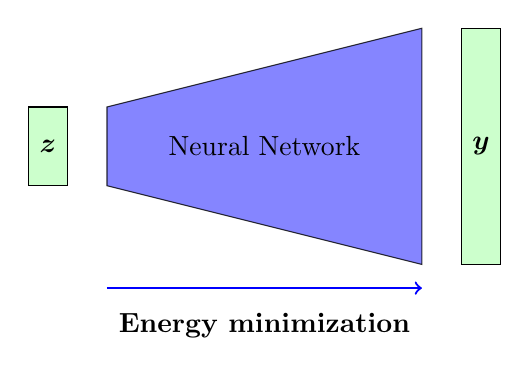
\begin{tikzpicture}
        % Modal coordinate (z)
        \draw[fill=green!20] (-3, 1) rectangle (-2.5,2);
        \node at (-2.75, 1.5) {$\bm{z}$}; % Label inside the rectangle
        
        % Displacement (u)
        \draw[fill=green!20] (2.5,0) rectangle (3,3);
        \node at (2.75, 1.5) {$\bm{y}$}; % Label inside the rectangle
        
        % Energy loss transition
        \draw[fill=blue!60,opacity=0.8] (-2,1) -- (2,-0) -- (2,3) -- (-2,2) -- cycle;
        \node at (0,1.5) {Neural Network};
        \node[below] at (0,-0.5) {\textbf{Energy minimization}};
        
        % Energy loss arrow
        \draw[thick,blue,->] (-2,-0.3) -- (2,-0.3);
    
    \end{tikzpicture}
    \caption{Neural Modes architecture for learning nonlinear deformation corrections}
    \label{fig:neural_modes_arch}
\end{figure}

\subsubsection{Training the Neural Modes}
The training process for the Neural Modes network is based on minimizing a combination of physics-based losses, rather than simply minimizing the prediction error against ground truth data. The key losses used in training are:

\begin{enumerate}
    \item \textbf{Energy Loss}: Minimizes the internal strain energy of the deformed configuration $E(\bm{X} + \bm{l} + \bm{y})$, where $\bm{X}$ is the rest position, $\bm{l}$ is the linear mode displacement given by $\bm{z}$, and $\bm{y}$ is the nonlinear correction.
    
    \item \textbf{Orthogonality Loss}: Ensures that the nonlinear correction is orthogonal to the linear mode space: $\bm{y}^T \bm{l} = 0$.
    
\end{enumerate}

The total loss function is a weighted sum of these individual losses:
\begin{equation}
    \text{Loss} = \text{Energy Loss} + \lambda_1 \text{Orthogonality Loss} + \lambda_2 \text{Origin Loss}
\end{equation}
where $\lambda_1$ and $\lambda_2$ are weight parameters that balance the importance of each loss term.

During the training process, it was observed that the network had the tendency to learn a correction when given \(z = 0\) (i.e., the rest position), and that was not intended, because the rest position should not have any correction, meaning that the model prediction should be zero. To avoid this, the network was designed to have zero bias, so that its output was centered at the origin.

\subsubsection{Dynamic Simulation with Neural Modes}
For dynamic simulations, the Neural Modes framework solves an optimization problem at each time step. Given the current and previous displacement states $\bm{u}_n$ and $\bm{u}_{n-1}$, the modal coordinates for the next time step $\bm{z}_{n+1}$ are computed by:
\begin{equation}
    \bm{z}_{n+1} = \underset{\bm{z}}{\argmin} \frac{1}{2h^2} \|\bm{n}(\bm{z}) - 2\bm{u}_n + \bm{u}_{n-1}\|_{\bm{M}}^2 + E(\bm{n}(\bm{z}))
\end{equation}
where $\bm{n}(\bm{z})$ represents the complete displacement field (linear modes plus nonlinear correction), $h$ is the time step, $\bm{M}$ is the mass matrix, and $E(\cdot)$ is the internal energy of the configuration. This optimization problem is typically solved using the L-BFGS-B algorithm.

One challenge with this approach is that the optimization problem does not explicitly account for external forces. The network learns to minimize internal energy but lacks direct information about external forces that may be applied during simulation. This limitation can affect the accuracy of dynamic simulations, particularly for large deformations or complex loading conditions.

\subsection{Extensions and Improvements}
A possible extension to the Neural Modes approach is to incorporate information about external forces directly into the network. This could be achieved by learning a mapping $\Phi: \mathbb{R}^m \rightarrow \mathbb{R}^n$ that relates modal coordinates $\bm{z}$ to the corresponding external forces $\hat{\bm{f}}$ that would produce such deformation. This additional network could be trained on a dataset of deformations and corresponding external forces, and then integrated into the dynamic simulation process to improve accuracy.

The objective function for dynamic simulation could then be extended to:
\begin{equation}
    \bm{z}_{n+1} = \underset{\bm{z}}{\argmin} \frac{1}{2h^2} \|\bm{n}(\bm{z}) - 2\bm{u}_n + \bm{u}_{n-1}\|_{\bm{M}}^2 + E(\bm{n}(\bm{z})) + \text{F}(\bm{z}, \bm{f})
\end{equation}
where $\text{F}(\bm{z}, \bm{f})$ is a term that accounts for the external forces acting on the system.

\section{Numerical Results}
\label{sec:numerical_results}
To verify the performance of the proposed method we test it on two different 3D problems based on two different geometries: a cantilever beam and the Stanford bunny. Both geometries use material properties designed to mimic soft tissue behavior, with Young's modulus $E = 10^6$ Pa and Poisson's ratio $\nu = 0.45$. \\

%\subsubsection*{Cantilever beam}
%\label{sec:cantilever_beam_setup}
The first test case is a cantilever beam with a square cross-section of size $1 \times 1$ and a length of $10$. The beam is clamped at one end and free at the other. This geometry represents a classical benchmark problem in structural mechanics, allowing for clear interpretation of the modal behavior and providing a controlled environment to validate the capabilities of our neural network approach. The cantilever beam exhibits well-understood physics with distinct modal patterns: bending modes in two perpendicular directions, torsional modes, and higher-order coupled deformation modes. The soft tissue material properties result in large deformations under relatively small loads, making this an ideal test case for nonlinear mechanics validation. \\

%\subsubsection*{Stanford bunny}
%\label{sec:stanford_bunny_setup}
The second test case employs the Stanford bunny \cite{bunny-mesh}, a widely recognized benchmark geometry in computational mechanics and computer graphics (see Figure \ref{fig:stanford_bunny}). This complex 3D shape presents a significantly more challenging validation scenario due to its intricate surface topology, non-uniform geometry, and irregular mass distribution. The Stanford bunny is fixed at its base and subjected to various loading conditions to generate the training data for the POD-based model reduction. This geometry tests the robustness and generalization capabilities of our method on realistic, non-trivial shapes that are commonly encountered in biomedical engineering applications. The complex geometry introduces coupling between different deformation modes and provides a stringent test for the neural network's ability to capture intricate displacement patterns typical of soft biological tissues. 

\begin{figure}[H]
    \centering
    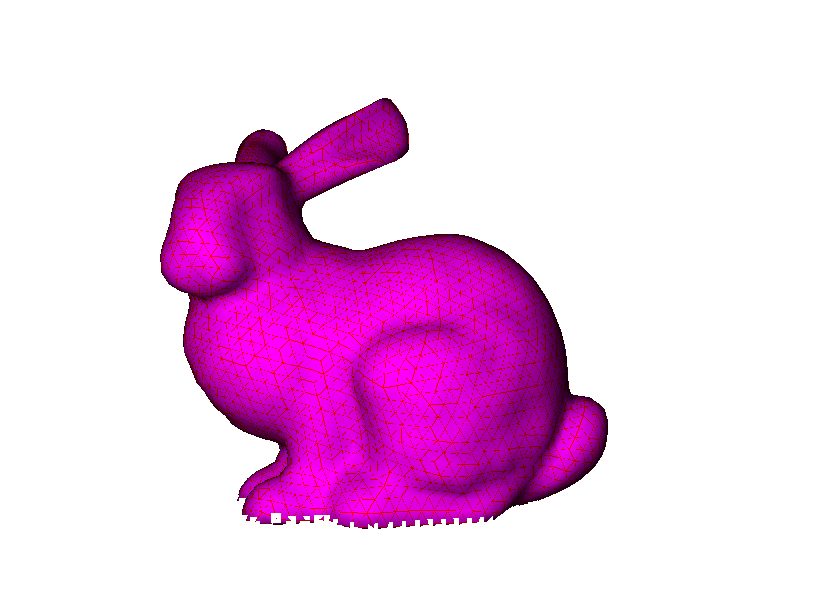
\includegraphics[width=0.7\textwidth]{Images/stanford_bunny.png}
    \caption{The Stanford bunny geometry used in the numerical test cases.}
    \label{fig:stanford_bunny}
    \end{figure}

Both geometries are discretized using tetrahedral finite elements, with mesh refinement studies performed to ensure convergence of the full-order solutions. The cantilever beam uses approximately 800 elements, while the Stanford bunny requires around 22000 elements.

\subsection{Optimal number of modes}
\label{sec:optimal_number_modes}
One of the first steps is clearly to determine the optimal number of modes to be used in the approximation. Using a low number of modes compromises the ability of reconstruction of the model, while choosing a number of modes that is too high, means that the complexity of the model increases, but the ability to reconstruct the displacement field doesn't increase much. The figure \ref{fig:optimal_number_modes} shows the error in the approximation of the displacement field as a function of the number of modes used. The error is computed as the Root Mean Square Error (RMSE) \eqref{eq:rmse}between the displacement field computed with the full model and the one computed with the reduced model. Figure \ref{fig:optimal_number_modes} shows that the error decreases rapidly with the number of modes used, and then stabilizes around 20 modes. We can see that with 10 modes the error is already below \(10^{-3}\) and with 20 modes the error is below \(10^{-4}\). For our use case, 7 modes are sufficient.
\begin{figure}[H]
    \centering
    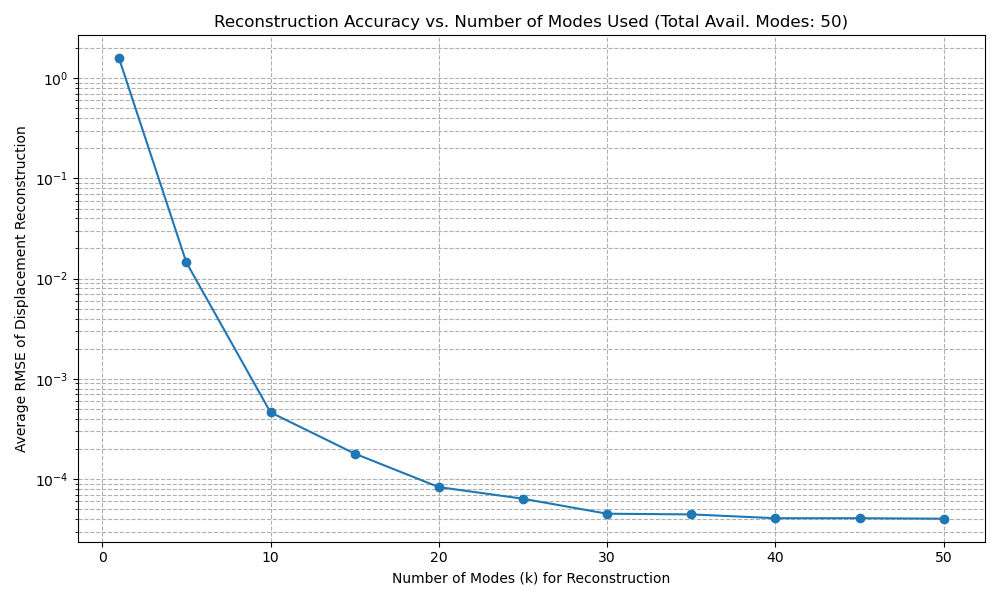
\includegraphics[width=0.7\textwidth]{Images/rmse_vs_modes.png}
    \caption{RMSE of the displacement field as a function of the number of modes used.}
    \label{fig:optimal_number_modes}
\end{figure}

\subsection{Training the model}
\label{sec:training_model}
The next step is to train the model using a supervised learning approach. For this purpose, we generate comprehensive datasets of labeled training examples for both geometries. The training data consists of triplets $(\mathbf{z}, \mathbf{u}, E_{FEM})$ where $\mathbf{z}$ represents the modal coordinates vector, $\mathbf{z}$ is the corresponding displacement field, and $E_{FEM}$ is the associated mechanical energy of the deformed configuration.
For the cantilever beam, we create a dataset of 600 deformations by applying different combinations of modal forces, described by a vector \(\mathbf{q}\) to the structure while maintaining the fixed boundary condition at one end. 


For the Stanford bunny geometry, we generate a dataset of 500 deformations using a similar sampling strategy. The modal coefficient ranges are determined based on preliminary analysis of the bunny's natural vibration modes and their relative contribution to physically realistic deformations.

Each training sample is generated by first selecting a random combination of modal coordinates within the specified ranges, then computing the corresponding displacement field and total mechanical energy using the full-order FEM solver. This supervised approach ensures that the neural network learns from accurate, physics-based ground truth data.

The neural network is trained to simultaneously predict both the displacement field and the mechanical energy given the modal coordinates as input. This multi-output formulation allows the model to learn the coupled relationship between geometric deformation and energy, which is crucial for maintaining physical consistency during predictions. The network architecture consists of fully connected layers with appropriate activation functions to capture the nonlinear mapping from modal space to the physical displacement and energy fields.

The training process is described in detail in Section \ref{sec:training_neural_modes}.

For the cantilever beam, we stopped the training, after 200 epochs, when the loss reached a plateau and we observed no significant improvement in the last 50 epochs. In Figure \ref{fig:training_loss_beam} we can see the training loss for the cantilever beam, which shows that immediately after the first epoch the loss drops significantly, meaning that the model is able to learn the underlying physics of the problem very quickly. We then let the model train until epoch 200 so that it can receive as input a wide range of different configurations and be able to generalize well.

\begin{figure}[H]
    \centering
    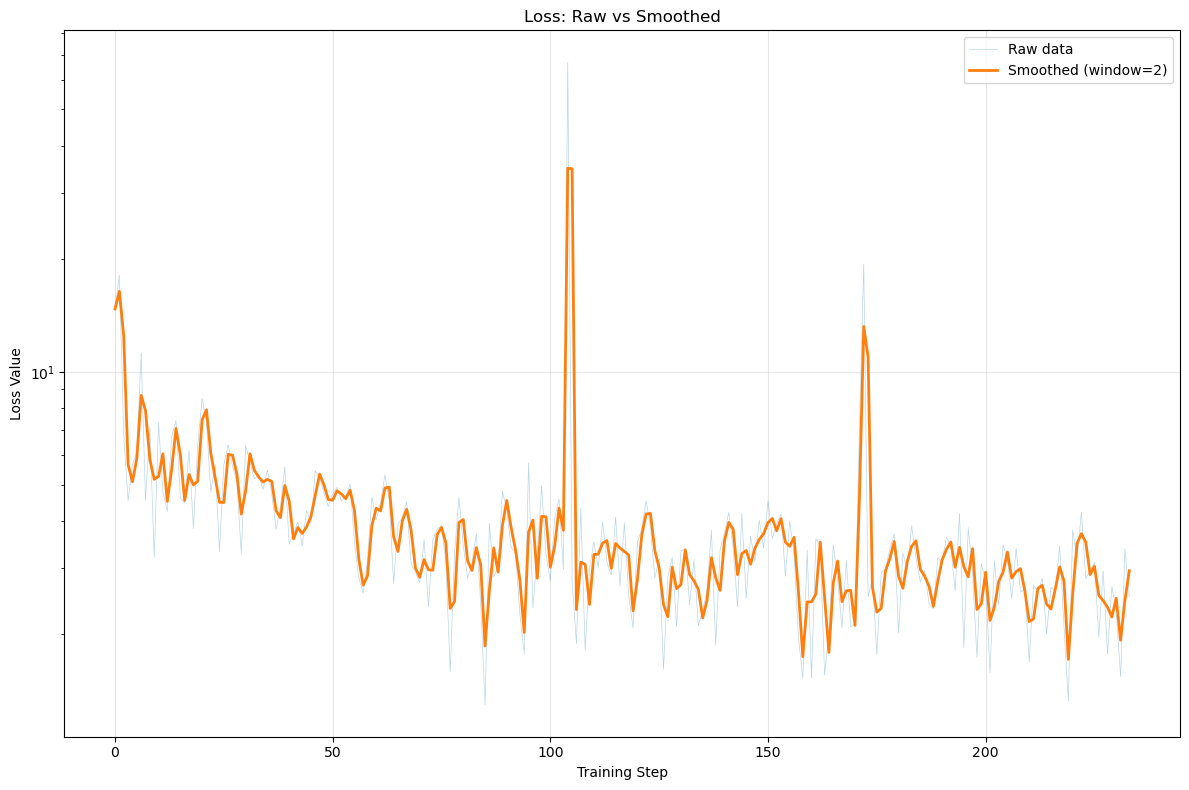
\includegraphics[width=0.7\textwidth]{Images/training_loss_smoothed_logy.png}
    \caption{Training loss for the cantilever beam.}
    \label{fig:training_loss_beam}
\end{figure}

We also provide the plot of the energy part of the loss function, which is computed as the mean of the internal energy of the batch of training samples. As we can see in Figure \ref{fig:training_energy_loss_beam}, at the first epoch the energy is very high, because the last layer of the neural network is set to have zero weights and biases, meaning that at the end of first epoch the prediction is just the linear modes approximation, then the energy loss drops significantly in the first few epochs, learning a meaningful correction to the linear modes approximation, while maintaning the ability to generalize even though the training set is not very large. The energy loss stabilizes around \(5e3\), which is on par with the energy computed in the validation phase with the full-order FEM solver.

\begin{figure}[H]
    \centering
    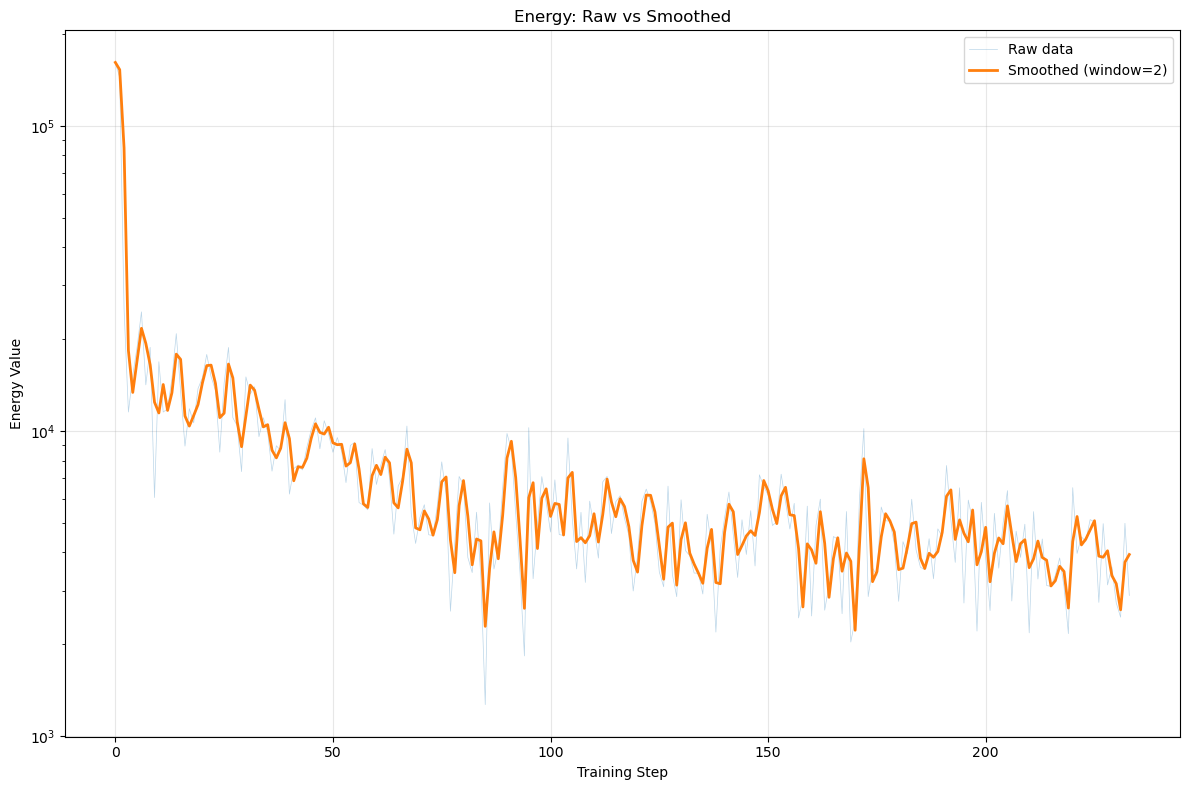
\includegraphics[width=0.7\textwidth]{Images/training_energy_smoothed_logy.png}
    \caption{Training energy loss for the cantilever beam.}
    \label{fig:training_energy_loss_beam}
\end{figure}


\subsection{Model Validation}
\label{sec:model_validation}
We perform the validation of the proposed neural modes model in two main ways: evaluating its accuracy in reconstructing displacement fields for various static configurations and assessing its performance in predicting the time-dependent behavior in a dynamic problem. Additionally, for comparison, we evaluate an alternative approach based on self-supervised training.

\subsubsection{Evaluation of Self-supervised Model}
\label{sec:evaluation_self_supervised}
To provide insight into the effectiveness of the supervised training approach used for our primary model, we trained an alternative network following a self-supervised procedure described by \cite{Wang_Du_Coros_Thomaszewski_2024}. In this method, the network is trained solely by minimizing the energy loss function, without using any ground truth displacement data. The training is performed by sampling modal coefficients uniformly within the ranges established during the supervised training phase:
\begin{align*}
    z_1 &\in [-225, 225], \\
    z_2 &\in [-170, 170], \\
    z_3 &\in [-20, 20], \\
    z_4 &\in [-15, 15], \\
    z_5 &\in [-5, 5], \\
    z_6 &\in [-80, 80], \\
    z_7 &\in [-170, 170].
\end{align*}
We then perform the validation of this self-supervised model on the same static validation set used for the supervised training. The results are shown in Figure \ref{fig:self_supervised_validation_mse_comparison}, where we can see that the self-supervised model performs at most as well as the linear modes model in terms of displacement accuracy. This indicates that, for this problem, self-supervised training alone does not provide a significant advantage over the simpler linear modes approximation when evaluating displacement fields.

\begin{figure}[H]
    \centering
    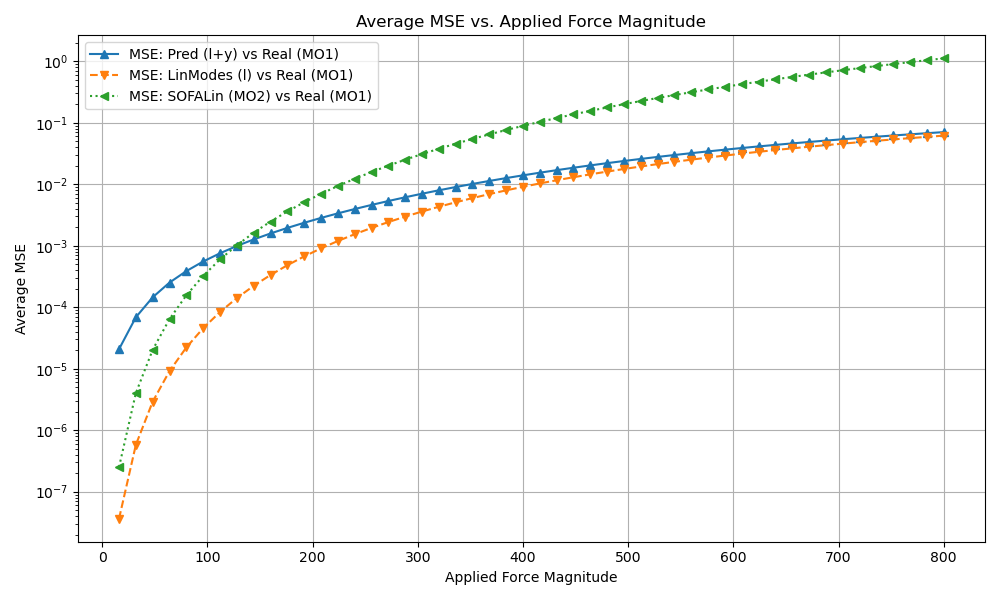
\includegraphics[width=0.8\textwidth]{Images/self_supervised_mse.png}
    \caption{Average MSE comparison for the self-supervised neural modes model (blue) against the linear modes model (orange) and the linear FEM model (green), evaluated against the nonlinear FEM ground truth. The self-supervised model performs similarly to or worse than the linear modes in terms of displacement accuracy.}
    \label{fig:self_supervised_validation_mse_comparison}
\end{figure}

As we can see, the self-supervised model does not even reach the performance of the linear modes model, which is a clear indication that the self-supervised training approach is not ideal to our problem. Now we can proceed to show the results of the supervised neural modes model, both in static and dynamic validation scenarios.

\subsubsection{Static Validation}
\label{sec:static_validation}
For the static validation phase, we test the supervised neural network model's ability to accurately reconstruct displacement fields for various static configurations that were not seen during training. This validation is crucial to establish confidence in the model's interpolation capabilities within the trained parameter space and to verify that the network has successfully learned the underlying physics of the structural mechanics problem. The results of this static validation, including quantitative comparisons (MSE, energy) and qualitative visualizations, are presented immediately following this section. 


We generate a comprehensive test dataset consisting of 100 random static configurations by sampling modal coefficients uniformly within the established training ranges for each mode. Each test case represents a unique static equilibrium state of the cantilever beam under different loading conditions. For each configuration, we compute the reference displacement field using the full-order FEM solver and compare it with the neural network's prediction. The comparison is performed both qualitatively through visual inspection of the displacement fields and quantitatively using the Root Mean Square Error (RMSE) metric. As a benchmark we provide the reconstruction done by projecting the full displacement onto the reduced subspace (what we call ``linear modes'') and the full FEM model equipped with linear elasticity.

At 800N of applied force, the maximum MSE is $10^{-3}$ for the neural model, significantly outperforming both the linear modes model ($10^{-3}$) and the FEM with linear elasticity ($10^{-2}$). The maximum observed error across all test cases is $1.2 \times 10^{-3}$, while the minimum is $1.2 \times 10^{-5}$, demonstrating that the model maintains excellent accuracy across the entire range of test configurations. Importantly, the neural network error remains bounded within this narrow range ($10^{-5}$ to $10^{-3}$) across all force magnitudes, making it significantly more reliable than linear modes, which perform very well for small displacements but exhibit exponentially growing errors when operating outside the small deformation range. These results confirm that the neural network has successfully learned to approximate the complex nonlinear relationship between modal coordinates and the resulting displacement fields with remarkable precision and consistent reliability.

Figure \ref{fig:static_mse_comparison} presents the average MSE comparison between three different approaches: neural modes, linear modes, and linear FEM, all evaluated against the nonlinear FEM ground truth across force magnitudes ranging from $0$ to $800$ $N$. The results reveal distinct performance characteristics across different deformation regimes. For small displacements in the linear range (low forces), the linear modes approach demonstrates superior accuracy due to its exact representation of the underlying linear physics. However, as the applied forces increase and the system enters the nonlinear deformation regime, the neural modes approach significantly outperforms both linear methods by approximately an order of magnitude. This performance crossover occurs around 100 N, where the geometric nonlinearities become dominant. The superior performance of neural modes in the nonlinear range validates the method's ability to capture complex deformation patterns that cannot be represented by linear modal decomposition alone.

\begin{figure}[H]
    \centering
    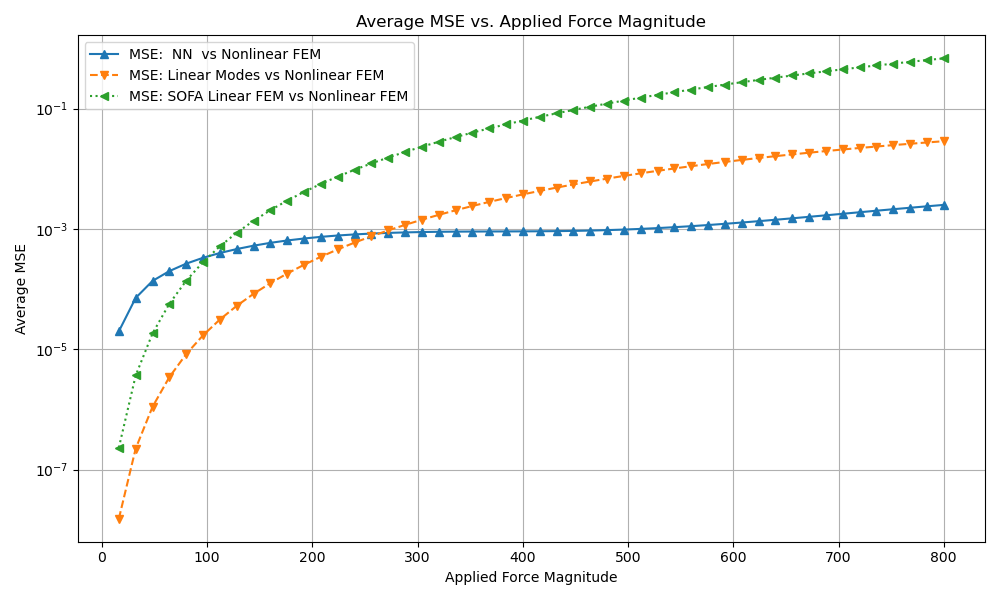
\includegraphics[width=0.8\textwidth]{Images/beam_static_mse.png}
    \caption{Average MSE between 100 different simulations with randomly applied forces. The neural modes model (blue) is compared against the linear modes model (orange) and the linear FEM model (green), all evaluated against the nonlinear FEM ground truth. The neural modes model significantly outperforms the linear modes, especially in the nonlinear regime.}
    \label{fig:static_mse_comparison}
\end{figure}

To provide additional insights into the model's performance, Figure \ref{fig:static_energy_beam} illustrates the relationship between the applied force and the internal mechanical energy of the beam. The graph compares the energy computed by the neural network model against the ground truth obtained from the nonlinear FEM solution. As we can see, in the small deformation regime, the linear modes outperform the neural modes, keeping the internal energy closer  to the ground truth. However, as the applied force increases and the beam undergoes larger deformations, the neural modes model manages to correct the linear model into a lower energy state, which is closer to the ground truth even in the case of large deformations. 
\begin{figure}[H]
    \centering
    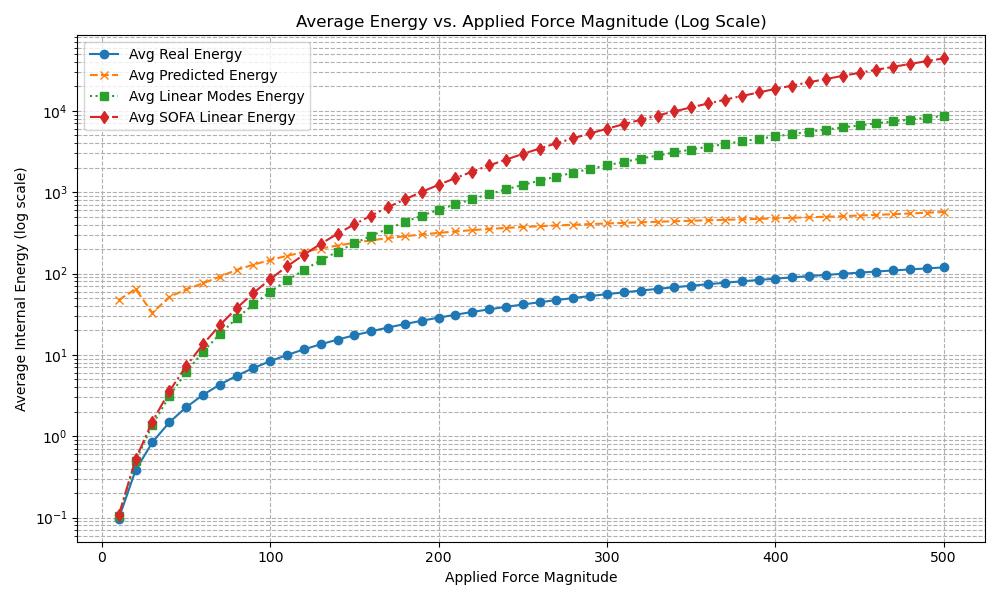
\includegraphics[width=0.8\textwidth]{Images/beam_static_energy.png}
    \caption{Internal mechanical energy of the beam as a function of the applied force. The blue line represents the energy computed by the neural network model, while the red line is the ground truth obtained from the nonlinear FEM solution. The green line represents the energy computed by the FEM with linear elasticity and the orange line is the energy computed by the linear modes model.}
    \label{fig:static_energy_beam}
\end{figure}


Figure \ref{fig:static_rmse_distribution} provides a detailed visual comparison of the different modeling approaches applied to a representative beam deformation case. In this visualization, we can observe the predicted deformation patterns from four different computational methods: the neural network prediction (shown in magenta), the ground truth nonlinear FEM solution (displayed in green), the linear modes approximation (represented by the red wireframe), and the linear FEM model (illustrated by the blue wireframe). 

This particular example demonstrates a critical limitation of linear approaches when dealing with large deformations. The linear modes and linear FEM models tend to significantly underestimate the pronounced bending curvature that develops in the beam under substantial loading conditions. The accentuated bending behavior observed in the ground truth solution is a characteristic manifestation of geometric nonlinearity, where the deformed configuration significantly influences the structural response.

However, the neural mode approach successfully captures this complex non-linear deformation pattern with remarkable accuracy. The magenta neural network prediction closely follows the green ground truth solution, demonstrating the model's capability to learn and reproduce the relationships between modal coordinates and the resulting nonlinear displacement fields. This superior performance in capturing geometric nonlinearities represents one of the key advantages of the proposed neural modes' methodology over traditional linear model reduction techniques, particularly for applications involving soft tissues and other materials that undergo large deformations during normal operation.

\begin{figure}[H]
    \centering
    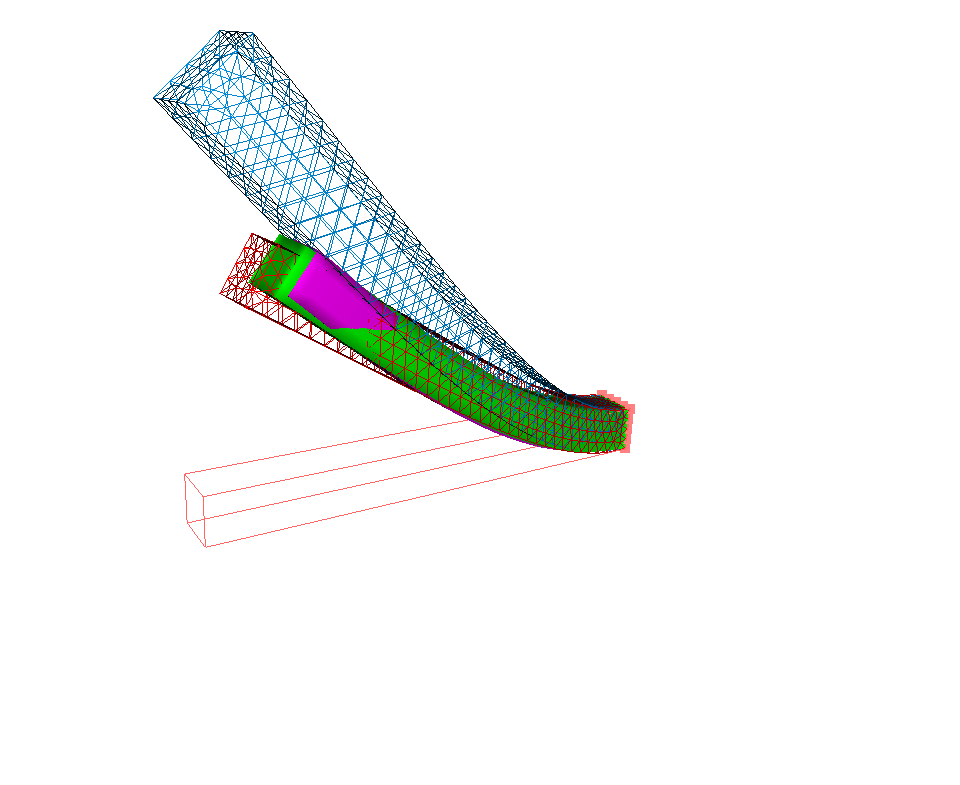
\includegraphics[width=0.4\textwidth]{Images/sofa_example_beam.png}
    \caption{Example of a static reconstruction in the case of the beam. The magenta beam represents the neural network prediction, the green one is the ground truth, the red wireframe represents the linear modes and the blue wireframe is the linear FEM model.}
    \label{fig:static_rmse_distribution}
\end{figure}

In the case of the Stanford bunny, the static validation follows a similar procedure. We generate a test dataset of 50 random configurations by sampling modal coefficients uniformly within the ranges established during training. Each configuration is then processed through the neural network to obtain the predicted displacement field, and grouped by the corresponding force applied to the bunny. The neural network's predictions are compared against the reference displacement fields computed using the full-order FEM solver discretizing the Neo-Hookean hyperelastic model, the linear modes approximation, and the linear FEM model.

Figure \ref{fig:static_mse_bunny} presents the average MSE comparison between the neural modes, linear modes, and linear FEM approaches across different force magnitudes applied to the Stanford bunny. The results reveal a similar trend to that observed in the cantilever beam case. In this case we observe a significantly better reconstruction using the Neural Modes, except for a slight range of forces between 125 and 150 N where linear modes significantly outperforms it. Outside that small range the neural network achieves an improvement in accuracy of an order of magnitude compared to linear modes, demonstrating its ability to capture complex nonlinear deformation patterns that are not adequately represented by linear modal decomposition. 
\begin{figure}[H]
    \centering
    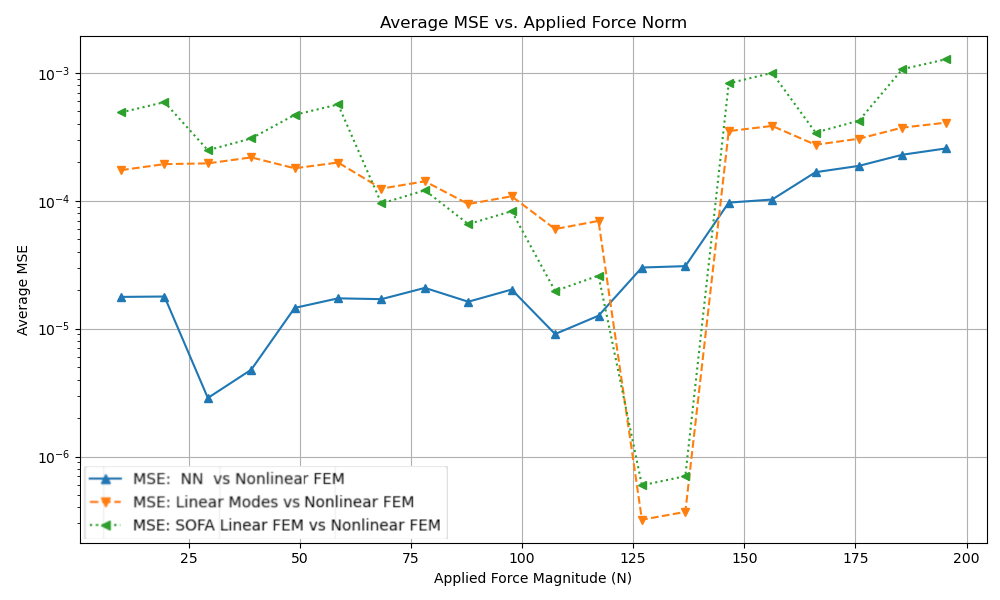
\includegraphics[width=0.95\textwidth]{Images/bunny_static_mse.png}
    \caption{Average MSE between 50 different simulations with randomly applied forces on the Stanford bunny. The blue line represents the MSE between the Neural Modes model and the nonlinear FEM, the orange line represents the MSE between linear modes and nonlinear FEM and the green one the MSE between the linear FEM and the nonlinear FEM}
    \label{fig:static_mse_bunny}
    \end{figure}

Also in this case, Figure \ref{fig:static_energy_bunny} illustrates the relationship between the applied force and the internal mechanical energy of the object. Again, we have energies that are lower by an order of magnitude than the linear modes and two orders of magnitude lower than the linear FEM model. In the case of the bunny the energy datum is particularly important, as the principal modes of deformation of the object are related to his head and ears, which means that most of its body is not deformed, keeping the MSE between the predicted displacement field and the ground truth very low, even if the prediction is far from being correct. Having that many nodes that stay still even in the deformed configuration, calls for additional metrics to evaluate the performance of the model, such as the internal energy, which we observe has a tendency to explode using linear elasticity or a combination of linear modes, but in the case of the neural modes model, the energy is at most two order of magnitude higher than the ground truth in the worst case scenarioscritti p, while the linear modes are consistently more than two order of magnitude higher than the nonlinear FEM.

\begin{figure}[H]
    \centering
    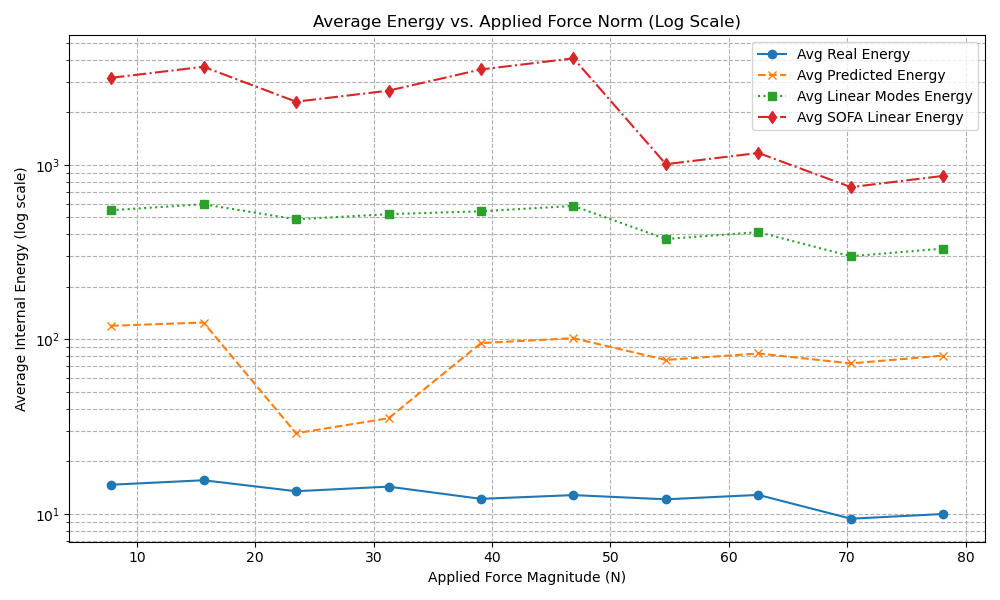
\includegraphics[width=0.8\textwidth]{Images/bunny_static_energy.png}
    \caption{Internal mechanical energy of the Stanford bunny as a function of the applied force. The blue line represents the energy computed by the neural network model, while the red line is the ground truth obtained from the nonlinear FEM solution. The green line represents the energy computed by the FEM with linear elasticity and the orange line is the energy computed by the linear modes model.}
    \label{fig:static_energy_bunny}
    \end{figure}
In  Figure \ref{fig:sofa_example_bunny} we can see an example of a static reconstruction in the case of the Stanford bunny. The magenta bunny represents the neural network prediction, the green one is the ground truth, the red wireframe represents the linear modes and the blue wireframe is the linear FEM model. As we can see, the force is applied  to the ears of the bunny, which are the most deformable parts of the geometry and exhibit a highly nonlinear behavior, as confirmed by the significant differences between the Neo-Hookean ground truth and the linear elasticity FEM model. The neural network prediction closely follows the ground truth, while the linear modes tends to amplify the volume of the ears and fail to reconstruct the bending behavior of them.

\begin{figure}[H]
    \centering
    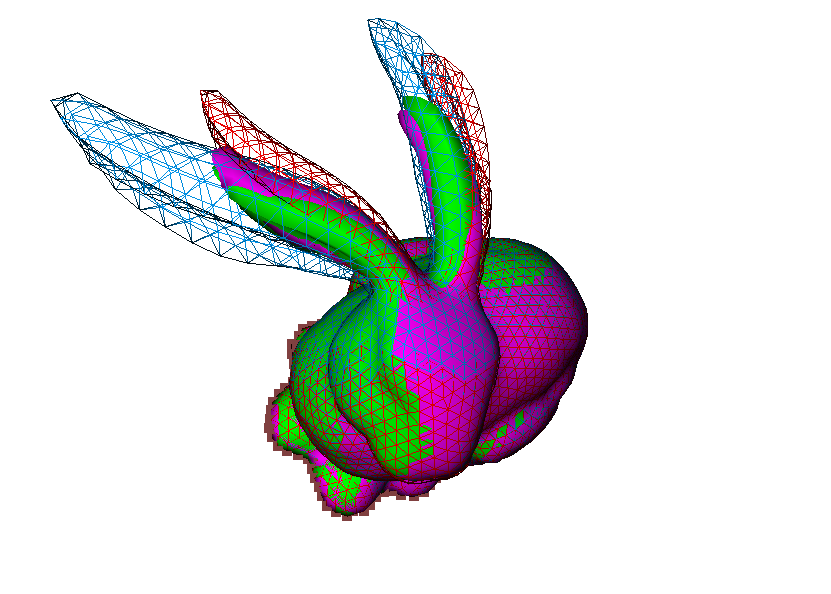
\includegraphics[width=0.4\textwidth]{Images/sofa_example_bunny.png}
    \caption{Example of a static reconstruction in the case of the Stanford bunny. The magenta bunny represents the neural network prediction, the green one is the ground truth, the red wireframe represents the linear modes and the blue wireframe is the linear FEM model.}
    \label{fig:sofa_example_bunny}
    \end{figure}
    
\subsubsection{Interpretability}
Another important aspect of this framework is its interpretability. While neural networks have a tendency to be completely black boxes, meaning that it is very hard to understand how a small change in the input can lead to a change in the output, in this case, the model is easily interpretable, since the input is a vector of coefficients that are then used to compute the displacement field using the modal basis. While linear modes are computed just as 
\begin{equation*}
    \bm{u} = \sum_{i=1}^n z_i \bm{\phi}_i,
    \end{equation*}
    the neural modes model computes the displacement field as
    \begin{equation*}
    \bm{u} = \sum_{i=1}^n z_i \bm{\phi}_i + \bm{f}(z),
    \end{equation*}
    where $\bm{f}(z)$ is the output of the neural network. This means that using a vector that has zero coefficients in all, but one of the modes, we can easily see how the neural network modifies the displacement field in that particular mode. This is a very important feature, since it allows us to understand how the neural network is modifying the displacement field in each mode, and how it is able to capture the nonlinear behavior of the system. 
    In Figure \ref{fig:latent_space_viz} we can see a visualization of the latent space of the neural modes model for the Stanford bunny and the 7 corresponding modes. We see that coefficients for the vector tend to decrease as we move from the first mode to the last one, which is on par with what we experienced when we faced the question of the optimal sampling of the latent space in Section \ref{sec:sampling_modal_space}.

\begin{figure}[H]
    \centering
    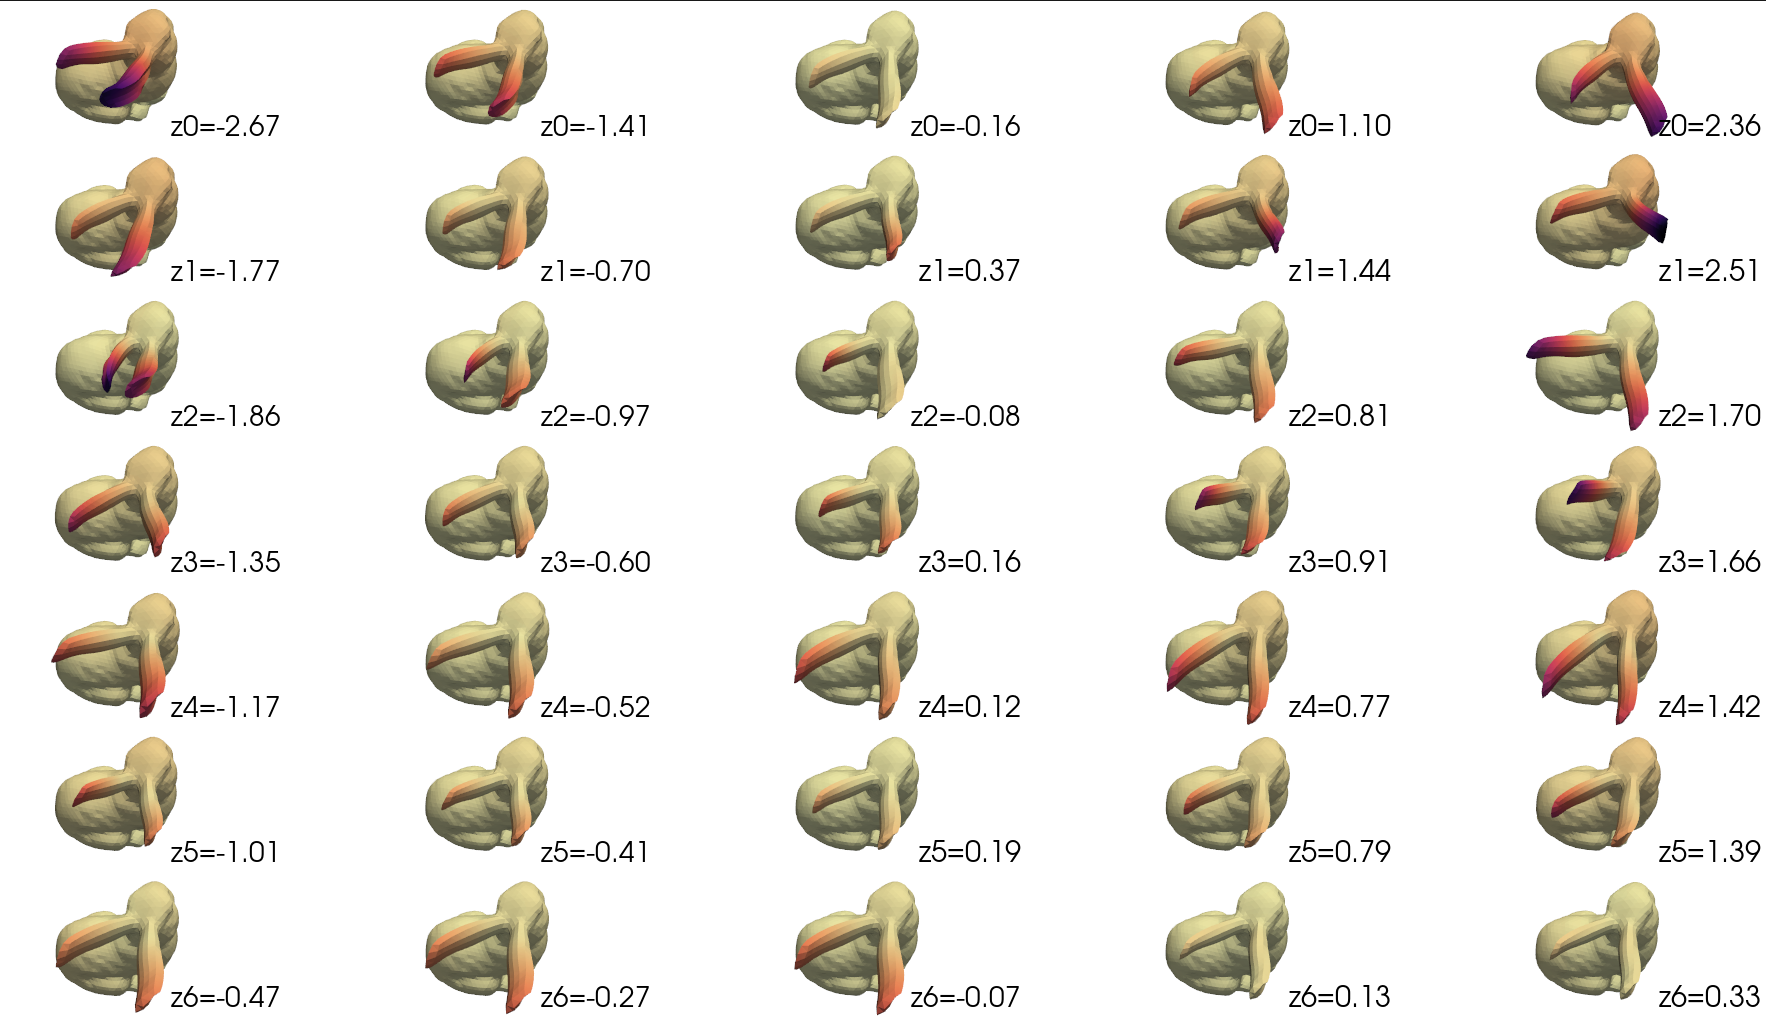
\includegraphics[width=\textwidth]{Images/latent_space_viz.png}
    \caption{Visualization of the latent space of the neural modes model for the Stanford bunny. Each row represents a different mode, and in the corner we can see the actual value of the coefficient for that mode.}
    \label{fig:latent_space_viz}
    \end{figure}
    

\subsubsection{Dynamic validation}
\label{sec:dynamic_validation}
The dynamic validation represents a more challenging and comprehensive test of the neural network model's capabilities, as it evaluates the model's performance in predicting time-dependent structural behavior over extended simulation periods. Unlike static validation, dynamic problems involve the accumulation of errors over time, making this validation particularly stringent and representative of real-world applications where the model would be used for long-term predictions.

For the dynamic validation procedure, we implement a hybrid approach where the first two time steps are computed using the full-order FEM solver to establish accurate initial conditions, including both displacement and velocity fields. Subsequently, we employ the neural network model in conjunction with the optimization problem defined in equation \eqref{eq:optimization_problem} to predict all subsequent time steps. This methodology allows us to assess how well the model can maintain physical consistency and accuracy when operating in a predictive mode over extended time horizons.

To obtain two time steps that are representative of the dynamic behavior of the system, our testing environment is set up to run the first 100 time steps with the FEM solver, and then take the last two time steps to initialize the neural network model. Then we integrate the neural network model in time by minimizing \eqref{eq:optimization_problem} until we see a significant divergence from the ground truth, which happens after around 120 steps. While this results seems less than ideal, it paves the way for future work to improve the underlying model and also fine tune the optimization problem to obtain a more accurate prediction.

As we can see from the  results, the neural network model performance in terms of MSE is just slightly better than the linear modes model, which raises questions about the need of  using a neural network for this problem. This is a perfectly valid concern, since the linear modes model is already a very good approximation of the displacement field, and it is much simpler to implement. As we can see in Figure \ref{fig:dynamic_validation_mse_comparison}, both the neural modes and linear modes models stray further from the ground truth as time progresses, but the neural modes model does slightly better, especially in the initial steps. When we reach the last part of the simulation, the MSE of the neural modes model is around 0.1, which clearly means that the prediction is not very accurate.

\begin{figure}[H]
    \centering
    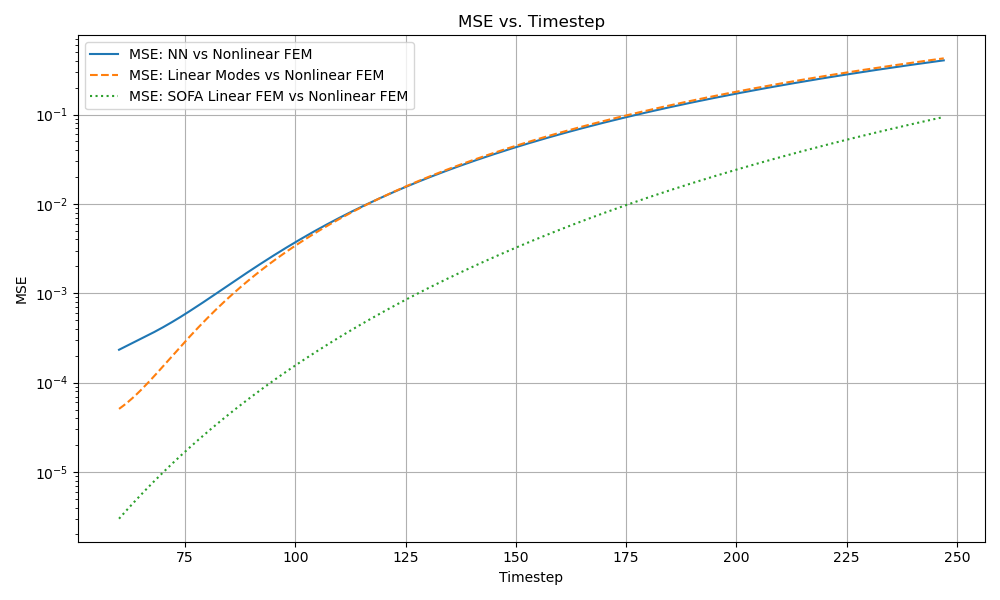
\includegraphics[width=0.8\textwidth]{Images/beam_dynamic_mse.png}
    \caption{MSE of the displacement field as a function of time for the dynamic validation of the cantilever beam. The neural modes model (blue) and the linear modes model (orange) are compared against the ground truth obtained from the nonlinear FEM solution (green). The neural modes model performs slightly better than the linear modes model, especially after the first few time steps.}
    \label{fig:dynamic_validation_mse_comparison}
    \end{figure}

Things change drastically when we take a look at the internal energy of the system, as we can see in Figure \ref{fig:dynamic_validation_energy_comparison}. The neural modes model manages to keep the energy at a level that is much closer to the ground truth, while the linear modes model diverges significantly from it. We have seen that in terms of MSE with respect to the ground truth the linear modes behaves almost identically to the neural network model, but looking at the energy values, we see that after 50 timesteps, the neural network is able to predict a sequence of deformations that is at most one order of magnitude higher than the nonlinear FEM, which allows for realistic simulations. The linear modes model, on the other hand, diverges from the ground truth in terms of energy, which is a classic limitation of linear models when dealing with large deformations. Outside the linear regime, linear models tend to ``explode'' in terms of energy and volume, due to the inherent shortcomings of linear elasticity in capturing the complex behavior of materials.

\begin{figure}[htb]
    \centering
    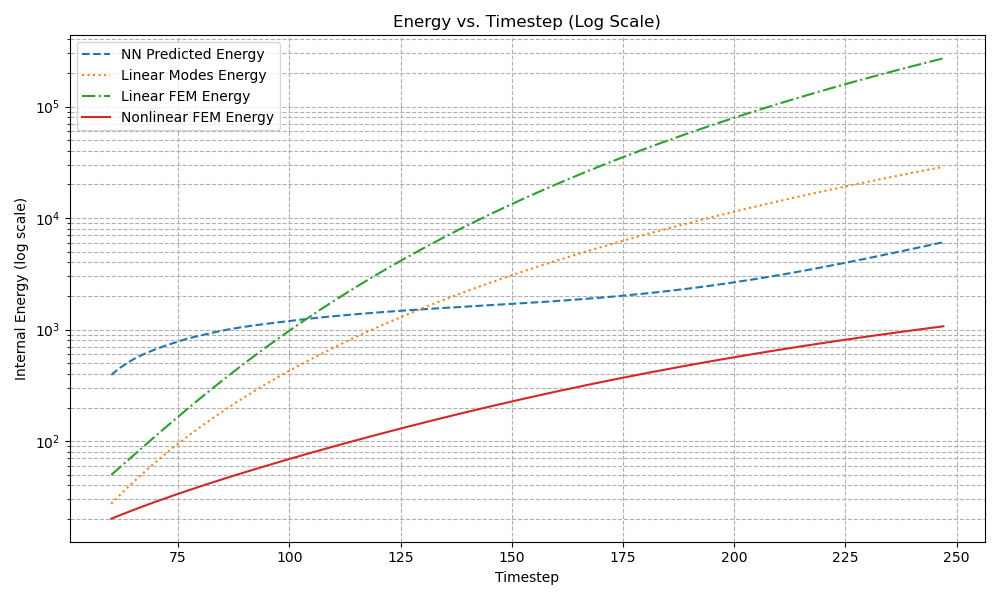
\includegraphics[width=0.8\textwidth]{Images/beam_dynamic_energy.png}
    \caption{Internal mechanical energy of the cantilever beam as a function of time for the dynamic validation. The neural modes model (blue) and the linear modes model (orange) are compared against the ground truth obtained from the nonlinear FEM solution (red). The neural modes model manages to keep the energy at a level that is much closer to the ground truth, while the linear modes model diverges significantly from it.}
    \label{fig:dynamic_validation_energy_comparison}
    \end{figure}

This will be discussed more thoroughly in the conclusions of this thesis, but the main problem lies in the way the dynamic problem is set up \eqref{eq:dynamic_problem}. Since it is using a quasi-Newton method to optimize a cost function to find the best trajectory in the reduced space, we are already adding errors by using L-BFGS. We can see that, once the network is trained, is able to produce realistic simulation, but we completely miss on the accuracy of those simulations. This opens up to future improvements to this work, like computing the trajectory of the modal coordinates directly with a reduced system of equations as will be suggested in the next section.


\FloatBarrier % Place this after the section where you want to stop floats from moving forward



%-----------------------------------------------------------------------------
% CONCLUSION
%-----------------------------------------------------------------------------

\section{Conclusion}
\label{sec:conclusion}
In this work, we have explored the Neural Modes framework, which combines the strengths of linear modal analysis and deep learning to simulate the nonlinear deformation of objects. After analyzing the original method and developing an implementation that allowed us to test this method with the aid of SOFA as a numerical solver, we have identified some limitations of the original method, such as the limited range of deformations that can be accurately captured with the self-supervised training approach and the optimal sampling of the latent space. To address these limitations in our use case, we have proposed a modified version of the Neural Modes framework that incorporates a supervised learning strategy, that uses a limited amount of data to train the network, coupled with a loss function that includes the physics-informed energy term. This approach allows the network to generalize even to large deformations with a small amount of data needed and allows to use a reduced order model to compute a full FEM simulation, which is crucial for real-time applications. The results of our numerical experiments demonstrate the effectiveness of the modified Neural Modes framework in accurately capturing the nonlinear deformation of objects, even in the presence of large deformations. 


\subsection{Computational Considerations and Performance}
Our implementation demonstrates significant computational advantages over traditional non-linear FEM approaches. The reduction from thousands of degrees of freedom to a handful of modal coordinates (typically 7-20 modes) represents a substantial decrease in computational complexity. This dimensionality reduction, combined with the neural network's ability to capture nonlinear corrections efficiently, enables real-time simulation of complex deformation scenarios that would otherwise require significant computational resources.

The training phase, while requiring an initial step for data generation and network optimization, must be performed only once for a given geometry and material configuration. Once trained, the network provides instantaneous corrections to linear modal predictions, making it highly suitable for interactive applications. The memory footprint of the trained network is minimal compared to storing high-resolution FEM solutions, making deployment feasible even on resource-constrained platforms.

\subsection{Limitations and Future Directions}
Despite promising results, several limitations need to be addressed. The current framework's dynamic simulation accuracy, while maintaining energy conservation, shows some deviation from ground truth displacement fields over extended time periods. Future work could explore more sophisticated temporal integration schemes or adaptive optimization strategies to improve long-term stability.


As described in \cite{Andersson_2021}, a promising direction for this work could be to completely modify the dynamics of the system, by using a fully reduced dynamic model, where we obtain \(\left[M\right]\) and \(\left[K\right]\) matrices that we obtain reducing the original matrices \(M\) and \(K\) with respect to the modal basis
\begin{equation}
    \left[M\right] = \left[\Phi\right]^T M \left[\Phi\right], \quad \left[K\right] = \left[\Phi\right]^T K \left[\Phi\right],
\end{equation}
where \(\left[\Phi\right]\) is the matrix of the modal basis. Then, projecting the displacement field \(\mathbf{u}\) onto the modal basis, we obtain the reduced displacement field \(\mathbf{q} = \left[\Phi\right]^T \mathbf{u}\). The reduced dynamic system can then be written as
\begin{equation}
    \left[{M}\right] \ddot{\mathbf{q}} + \left[{K}\right] \mathbf{q} = \mathbf{f},
\end{equation}
which can be solved using standard numerical methods and provide a more efficient way to obtain the trajectory of the system in the reduced space. Due to time constraints and software limitations, we were not able to explore this direction in this work, but it would be a natural extension of this framework. This would remove the use of a cost function that is optimized using a quasi-Newton method, which tend to accumulate numerical errors over time, and using a full dynamic model would allow to use a more robust numerical integration scheme, keeping the accuracy of the simulation higher.


\subsection{Final Remarks}
This framework still represents a significant step toward bridging the gap between computational efficiency and simulation accuracy in nonlinear mechanics. By leveraging the interpretability of modal analysis and the expressiveness of neural networks, we have demonstrated a method that maintains physical consistency while achieving computational performance suitable for real-time applications.

This paradigm could be extended to other areas of computational physics where similar trade-offs between accuracy and efficiency exist.

As we move forward, the ongoing development of these hybrid approaches will likely become increasingly important for enabling new applications that demand both accurate physics and real-time performance. The Neural Modes framework shows that well-designed machine learning can improve, rather than replace, core physical modeling principles.
%---------------------------------------------------------------------------
%  BIBLIOGRAPHY
%---------------------------------------------------------------------------
\newpage
\printbibliography
% Remember to insert here only the essential bibliography of your work
% automatically inserted and ordered with this command

\newpage
\textbf{Abstract italiano:} \abstractita

\begin{tcolorbox}[arc=0pt, boxrule=0pt, colback=bluePoli!60, width=\textwidth, colupper=white]
        \textbf{Parole chiave:} \keywordsita
    \end{tcolorbox}

\end{document}

